\documentclass[11pt]{article}
\usepackage{icmlko}
\begin{document}

\title{문을 열었더니 문이 하나 더 있었다 --- 부트스트랩이 두 번 걸린다}
\author{월드모델 실험실}
\date{노트 359 · 2026년 8월 1일}
\maketitle

\begin{abstract}
노트 358이 팝업 학습을 $16 \to 24$ 로 늘리면서 노트 281의 잎 문턱 22를
처음 넘겼다. 노트 276이 만들고 281이 ``문턱 아래라 죽는다''로 접은 팝업
전용 축 넷을 되살렸다. 붙는다 --- 열이 $34 \to 38$, 살아 있는 열이
$5 \to 9$ 다. \textbf{한 번 적합에서는 산다}: 팝업 $+0.0051$ · 판
$+0.0002$(노트 351의 환율이 $+0.0018$ 로 예측했다). \textbf{그런데 짝
열둘에서는 열 번이 바이트까지 같다} --- 판 $+0.0001$(2/12) · 팝업
$+0.0004$(2/12). 기제를 셌다: \textbf{부트스트랩이 두 번 걸린다.} 짝
규약이 학습 행을 재표집하고(서로 다른 행 63\%) F18 이 자루를 또
뽑는다(다시 63\%) --- $0.63^2 \approx 0.40$ 이라 팝업 24행이 자루 안
\textbf{9.8행}이 되고 잎 최소 20을 못 채운다. \textbf{노트 281의 법칙을
고친다} --- 문턱이 잎 최소 그 자체(22행)인 것은 \emph{한 번 적합}에서이고,
짝 규약 아래에서는 \textbf{50\textasciitilde{}65행}이 필요하다.
안 넣는다. 그리고 가는 길에 \textbf{여덟 번째 갈라진 목록}을 찾아 고쳤다 ---
노트 358이 만든 것이다.
\end{abstract}

\section{문이 열렸다}

노트 276이 팝업 전용 축 열여섯 중 넷을 남겼다(\texttt{pop\_comp} ·
\texttt{pop\_wkend} · \texttt{pop\_holid} · \texttt{pop\_stores}). 노트
281이 그것들이 왜 정확히 $+0.0000$ 인지 밝혔다 ---
\texttt{min\_samples\_leaf} 기본값 20 이고 팝업 학습이 16행이라 그 열로
가르는 분기가 \textbf{후보에도 못 오른다.} 문턱을 22로 확정했다.

노트 358이 등급 필터를 풀어 학습을 24로 만들었다. 처음으로 문턱 위다.
되살렸다. 붙는다 --- 팝업 열이 $34 \to 38$ 이고 표시자가 85\textasciitilde{}88\%다.

\textbf{그리고 가는 길에 여덟 번째 갈라진 목록을 찾았다.} 같은 거름망이
두 군데 적혀 있었다 --- \texttt{popupset.build(grades=...)} 와
\texttt{trendaxes.\_popup\_ids} 의 등급 목록이다. 노트 358이 앞쪽만
A\textasciitilde{}E 로 풀어서 뒤쪽은 A$\cdot$B 로 남았고, id 75건 대 자료
89행이라 \textbf{전용 축이 길이 불일치로 통째로 버려질 뻔했다.}
\texttt{set\_grades} 로 맞췄다. \textbf{노트 356이 ``같은 거름망이 두
군데 적혀 있으면 갈라진다''고 적었는데, 그 다음 노트가 바로 하나를
만들었다.}

\section{한 번 적합에서는 산다}

\begin{center}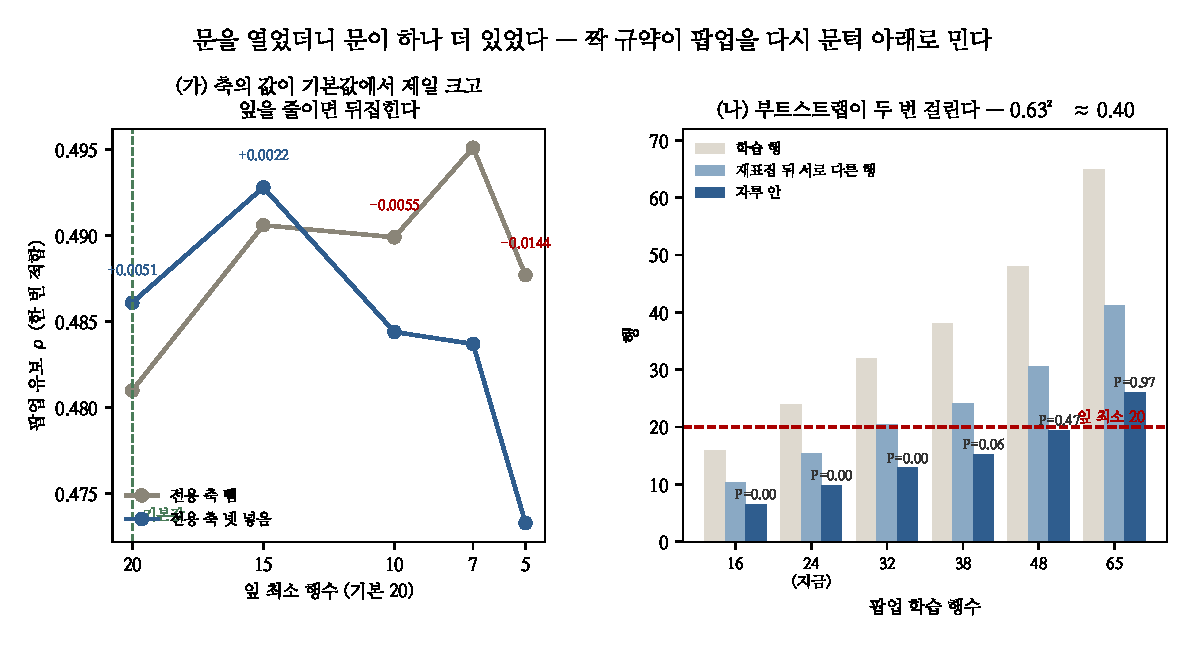
\includegraphics[width=\linewidth]{figs/twoboot.pdf}\end{center}

\begin{center}
\begin{tabular}{lrrr}
\hline
잎 최소 & 전용 축 뺌 & 넣음 & 축의 값 \\
\hline
\textbf{20}(기본) & 0.4810 & 0.4861 & $\mathbf{+0.0051}$ \\
15 & 0.4906 & 0.4928 & $+0.0022$ \\
10 & 0.4899 & 0.4844 & $-0.0055$ \\
7  & 0.4951 & 0.4837 & $-0.0114$ \\
5  & 0.4877 & 0.4733 & $-0.0144$ \\
\hline
\end{tabular}
\end{center}

\textbf{노트 276과 정반대다.} 그때는 $20 \to +0.0000$ · $10 \to +0.0394$ ·
$5 \to +0.4373$ 으로 잎을 줄일수록 살아났다. 지금은 기본값에서 제일 크고
줄일수록 뒤집힌다. 까닭은 그때와 지금이 다른 문제여서다 --- 16행 세상에서
잎을 줄이는 것은 \emph{그 열로 가르는 유일한 방법}이었고, 24행 세상에서는
이미 가를 수 있으니 잎을 줄이는 것은 \textbf{모두가 과적합하게} 두는 일일
뿐이다. 손해가 팝업 전용 축의 이득보다 크다.

(잎 7 에서 전용 축 없이 팝업이 0.4951 로 표에서 제일 높지만 \textbf{그걸
고르면 유보로 손잡이를 고르는 것이다} --- 노트 216 · 272 가 이미 세 번
막았다. 기본값 4$\cdot$20 을 안 건드린다.)

\section{짝에서는 죽는다}

\begin{center}
\begin{tabular}{lrrr}
\hline
 & 차 & SD & 부호 \\
\hline
판     & $+0.0001$ & 0.0001 & \textbf{2/12} \\
팝업   & $+0.0004$ & 0.0012 & \textbf{2/12} \\
나머지 여덟 & $\le +0.0004$ & --- & 0\textasciitilde{}3 / 12 \\
\hline
\end{tabular}
\end{center}

\textbf{열두 뽑기 중 열이 바이트까지 같다.} 노트 187의 값싼 검사다 ---
바꿨는데 안 움직이면 그건 ``효과가 없다''가 아니라 \textbf{모형에 안
닿은 것}이다.

\section{왜 --- 부트스트랩이 두 번 걸린다}

짝 규약은 \emph{학습 행을 재표집}한다. 부트스트랩 표본은 서로 다른 행을
$1-e^{-1} \approx 63\%$ 만 갖는다. 그리고 F18 은 쌓은 행렬에서 \emph{자루를
또} 뽑는다 --- 다시 63\%다. \textbf{둘이 곱해져 $0.63^2 \approx 0.40$ 이
된다.}

\begin{center}
\begin{tabular}{rrrr}
\hline
팝업 학습 & 재표집 뒤 다른 행 & 자루 안 & $P(\ge 20)$ \\
\hline
16 & 10.3 & 6.5 & 0.000 \\
\textbf{24}(지금) & 15.4 & \textbf{9.8} & \textbf{0.000} \\
32 & 20.4 & 12.9 & 0.004 \\
38 & 24.2 & 15.3 & 0.057 \\
48 & 30.6 & 19.4 & 0.475 \\
\textbf{65} & 41.2 & 26.1 & \textbf{0.973} \\
\hline
\end{tabular}
\end{center}

계산이 관측과 맞는다 --- 24행이면 자루 안 9.8 로 잎 최소 20의 절반이고,
실제로 열둘 중 둘만 움직였다.

\textbf{노트 281의 법칙을 고친다.}
\begin{quote}
문턱은 잎 최소 그 자체다(팝업 학습 22행) --- \textbf{한 번 적합에서.} \\
\textbf{짝 규약 아래에서는 $20/0.40 = 50$ 행이 필요하고, 거의 항상 살려면
65행이다.}
\end{quote}

노트 281이 웹툰 학습을 줄여 가며 문턱을 쟀는데 \emph{재표집 없이} 쟀다.
그래서 맞는 법칙을 \emph{한 번 적합}에 대해 얻었고, 실험실이 실제로 쓰는
눈금은 짝이다. \textbf{같은 종류의 어긋남이 노트 358에도 있었다} --- 한 번
적합의 도메인 칸이 짝과 부호부터 달랐다. 여기서는 문턱 자체가 다르다.

\section{안 넣는다 --- 그리고 다음 문}

노트 187의 검사가 걸렸으므로 넣을 근거가 없다. 팝업 전용 축은
\textbf{학습 65행}이 되기 전에는 이 규약 아래서 못 쓴다.

\textbf{그런데 65행이 손 닿는 데 있다.} 노트 357이 \texttt{organizer\_claim}
73행을 학습에 넣어 보고 손해($0.4905 \to 0.4514$)를 봤는데, 같은 글이
까닭도 밝혔다 --- 주장 라벨이 해마다 일정하게 부풀어 있다($+0.27$ ·
$+0.44$ · $+0.20$). \textbf{곱셈 부풀림은 기준 안에서 중앙을 빼면
사라진다.}

노트 357은 그 정규화를 ``과제를 바꾸는 결정''이라 미뤘는데,
\textbf{그것은 유보에 넣을 때의 얘기다.} 학습만 정규화하면 채점 집합이
그대로라 과제가 안 바뀐다 --- 노트 224의 규약이 막는 것은 \emph{라벨을
다시 정의해 점수를 바꾸는} 일이다. 학습 $24 \to 97$ 이면 65를 넉넉히
넘는다.

\section{남은 것}

\begin{center}
\begin{tabular}{ll}
\hline
갈래 & 지금 아는 것 \\
\hline
\textbf{주장 라벨 기준별 정규화(학습만)} & 팝업 학습 $24 \to 97$. 과제는 안 \\
 & 바뀐다. 그러면 전용 축이 산다. \textbf{다음 순번} \\
만화 2026 스무 건 & 노트 356. 열한 번째 채점 도메인 \\
만화가 왜 누르나 & 노트 356. 라벨 종류로는 안 갈린다 \\
잎 문턱을 도메인별로 & 지금은 전 도메인 공유다. 얇은 도메인만 \\
 & 낮추면? 노트 259의 ``복도'' 문제가 걸린다 \\
\hline
\end{tabular}
\end{center}

\end{document}
